%%% 本文档作为功能演示

\subsubsection{步兵机器人}

    %%% 长段演示-BEGIN
    第一段。\par
    
    第二段。\par
    
    第三段。\par
    %%% 长段演示-END

    \paragraph{需求分析}
    
        %%% 有序列表演示-BEGIN
        \begin{enumerate}
            \item 需求1。
        
            \item 需求2。
        \end{enumerate}
        %%% 有序列表演示-END
    
        %%% 插入公式演示-BEGIN
        \begin{align*}
            \Vec{OP} &= \frac{1}{2} ( \Vec{OB} + \Vec{OD} ) = \frac{1}{2} ( \Vec{OA} + \Vec{AB} + \Vec{OE} + \Vec{ED} ) \\
            |PC| &= \sqrt{|BC|^2 - |BP|^2} \\
            \Vec{OC} &= \Vec{OP} + |PC|\hat{PC} , ~{where}~ \hat{PC} \perp \hat{BP} \\
            \Rightarrow l &= |OC| \\
            \Rightarrow \varphi_0 &= \pi + \arctan(z_C, x_C) \\
        \end{align*}
        %%% 插入公式演示-END
        %%% 具体公式具体分析,公式排版很复杂,是一门学问
    
    \paragraph{设计思路}
        
        %%% 插入图片演示-BEGIN
        \begin{figure}[H]
            \centering
            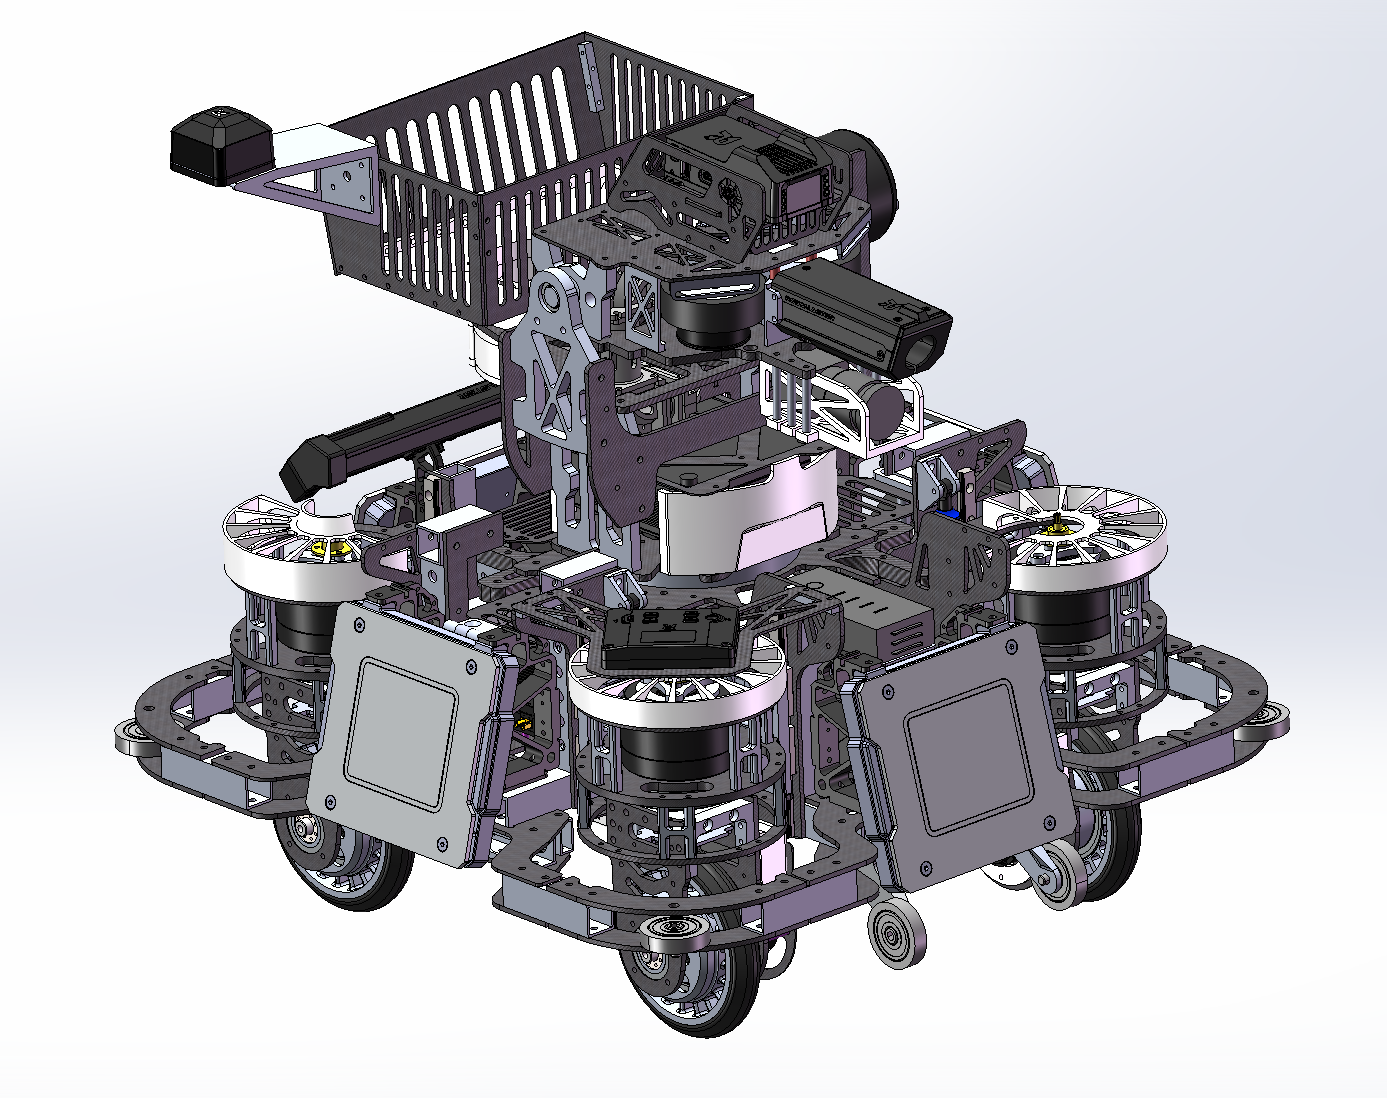
\includegraphics[height=0.35\textwidth]{figure/2_test1.png}
            \hspace{0.5em}
            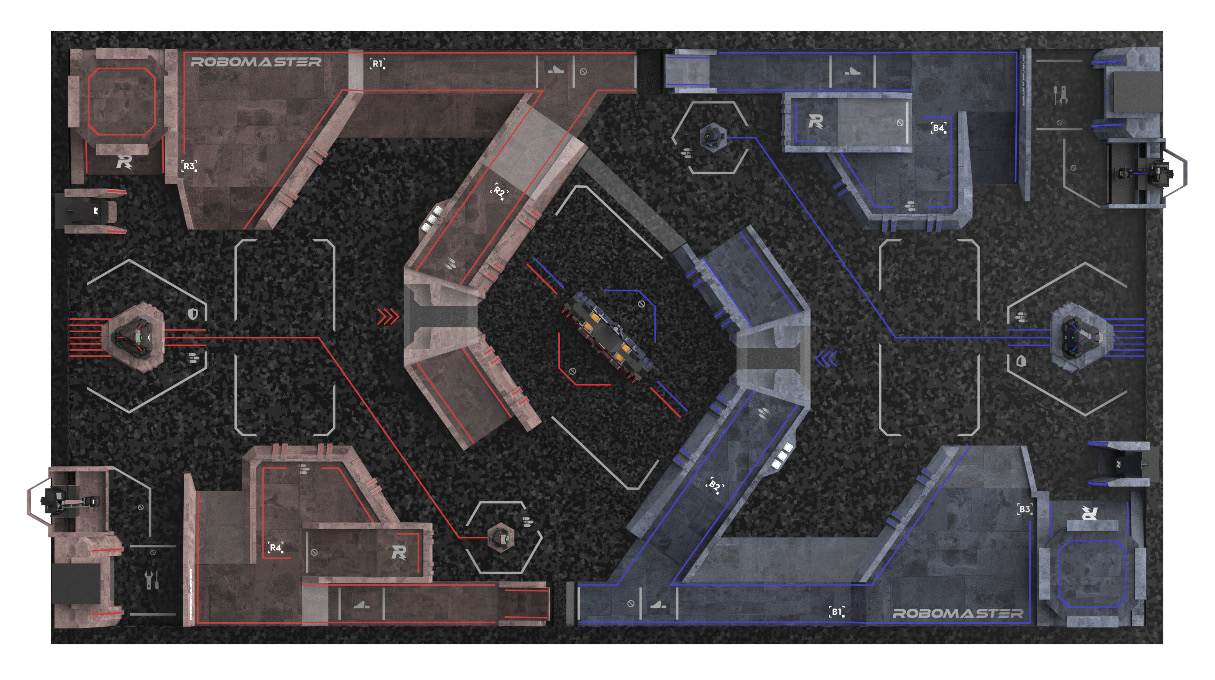
\includegraphics[height=0.35\textwidth]{figure/2_test2.png}
            \label{fig:test}
        \end{figure}
        %%% 插入图片演示-END
        %%% 图片居中放置
        %%% 该图片存储路径为 ./figure/2_test1.png 以及 ./figure/2_test2.png两张图
        %%% \label表示的是该图坐标位置,可以由其他地方引用跳转

    \paragraph{任务安排}
    
        %%% 插入图片引用演示-BEGIN
        点击此处跳转到四舵轮底盘图片处:
        \ref{fig:test}
        %%% 插入图片引用演示-END
        %%% fit:后面的内容为图片对应的label
        
        点击此处跳转到大疆官方比赛配件网站:
        %%% 插入网址引用演示-BEGIN
        \href{https://www.robomaster.com/}{RM官网}
        %%% 插入网址引用演示-END

        %%% 无需缩进的时候可以加一句整个
        \noindent
        
        %%% 插入表格演示-BEGIN
        \LTXtable{\textwidth}{table/2_insertTable_sample.tex}
        %%% 插入表格演示-END
        %%% 该表格存储路径为 table/2_插入表格示例.tex ,表格相关代码的具体内容可以打开该文件查看